\documentclass[10pt]{article}
\usepackage{graphicx}

\newcommand{\code}[1]{\texttt{#1}}

\title{DESI GFA metrology to on-sky pixel conversions}
\author{Dustin Lang}
\date{2019-11-25}

\begin{document}

\maketitle

The DESI GFAs underwent metrology at Berkeley Lab, using a setup that
allowed a dot to be projected onto the GFA CCD, which could then be
measured in physical coordinates and also observed by reading out the
GFA CCDs.  This allows the GFA pixel grid to be tied to a physical
coordinate system in which the GFA Illuminated Fiducials (GIFs) are
also measured.

This document interprets the lab report measurements in terms of the
way the GFA images are read out in operations on the mountain, in
support of predicting the on-sky positions of the GFAs, GIFs, and (via
FVC images) the other fiducials and fibers.

The GFA metrology procedure is documented in DESI-4782.  The resulting
measurements are presented with one document per GFA device, as
detailed in Table \ref{tab:gfareports}.  This table is listed in Petal
location order, looked up via DESI-5286v5.

\begin{table}[h!]
  \begin{center}
    \begin{tabular}{|c|c|c|c|c|c|}
      \hline
      Petal Location & GFA name & Petal ID & GFA ID & GFA Metrology doc & Petal Metrology doc \\
      \hline
      0 & GUIDE0 & 4  & GFA\#10 & DESI-4832-v2 & DESI-4900-v1 \\
      1 & FOCUS1 & 5  & GFA\#5 & DESI-4825 \\
      2 & GUIDE2 & 6  & GFA\#6 & DESI-4823 \\
      3 & GUIDE3 & 3  & GFA\#2 & DESI-4821 \\
      4 & FOCUS4 & 8  & GFA\#7 & DESI-4824 \\
      5 & GUIDE5 & 10 & GFA\#8 & DESI-4836 \\
      6 & FOCUS6 & 11 & GFA\#13 & DESI-4886 \\
      7 & GUIDE7 & 2  & GFA\#1 & DESI-4780 \\
      8 & GUIDE8 & 7  & GFA\#4 & DESI-4822-v3 \\
      9 & FOCUS9 & 9  & GFA\#3 & DESI-4837 \\
      \hline
    \end{tabular}
    \caption{\label{tab:gfareports}Installed locations of GFA devices and
      metrology report numbers.}
  \end{center}
\end{table}

In each GFA metrology report, there is a spreadsheet named
``GFA\#\#\_Lateral\_Measurements.xlsx'', plus a set of FITS images as a
zip file.  In the spreadsheet, the ``GFA Images'' tab has the spot
location measurements in millimeters, and GFA image filenames.  The
measured positions are only good to ~the nearest pixel, so we will
re-measure them with code.

The GFA images are FITS files with 4 image extensions, each $1106
\times 1056$ pixels.  NOTE that the FITS viewer \code{ds9} may not
show you the whole image by default---it may show only the active CCD
area, omitting the prescan and overscan columns, and the extra rows.
See Figure \ref{fig:metrologya}.  The extent of one-quarter of
the physical CCD area ($1024 \times 1032$) is shown.

\begin{figure}[h!]
  \begin{center}
    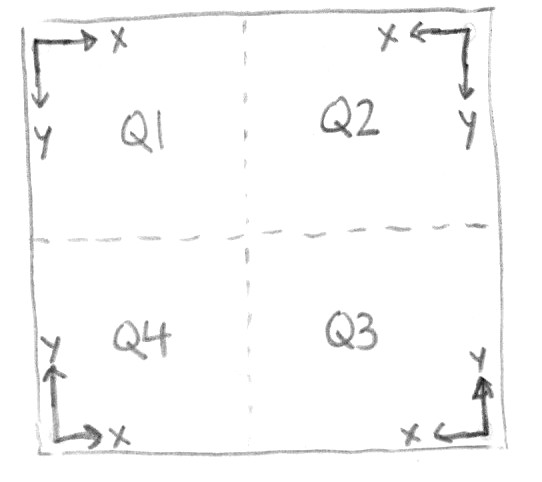
\includegraphics[width=0.3\textwidth]{gfa-metrology1a.jpeg}
    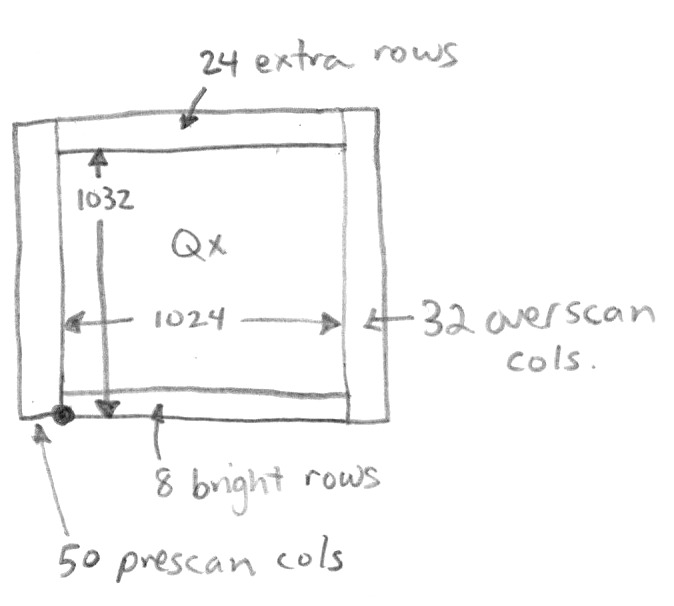
\includegraphics[width=0.5\textwidth]{gfa-metrology1b.jpeg}
  \end{center}
  \caption{\label{fig:metrologya}Left: layout of the four quadrants
    (with the same order as the FITS file extensions) in the GFA
    metrology images.  In the spreadsheets, the pixel locations of the
    spots are given in a combined coordinate system in the arrangement
    shown, with $(0,0)$ in the lower left. The axes mark the origin
    and direction of the pixels in each image.  Right: pixel layout
    within each FITS image.}
\end{figure}

On the mountain, the GFAs have a mask installed so that only the
central part of each CCD is illuminated, with the remaining chip area
used for frame transfer.  The \code{gfa*.fits.fz} files $2248 \times
1032$, with $50$-pixel prescan and overscan columns, leaving an
illuminated area of $2048 \times 1032$, as illustrated in Figure
\ref{fig:mountain}.

\begin{figure}[h!]
  \begin{center}
    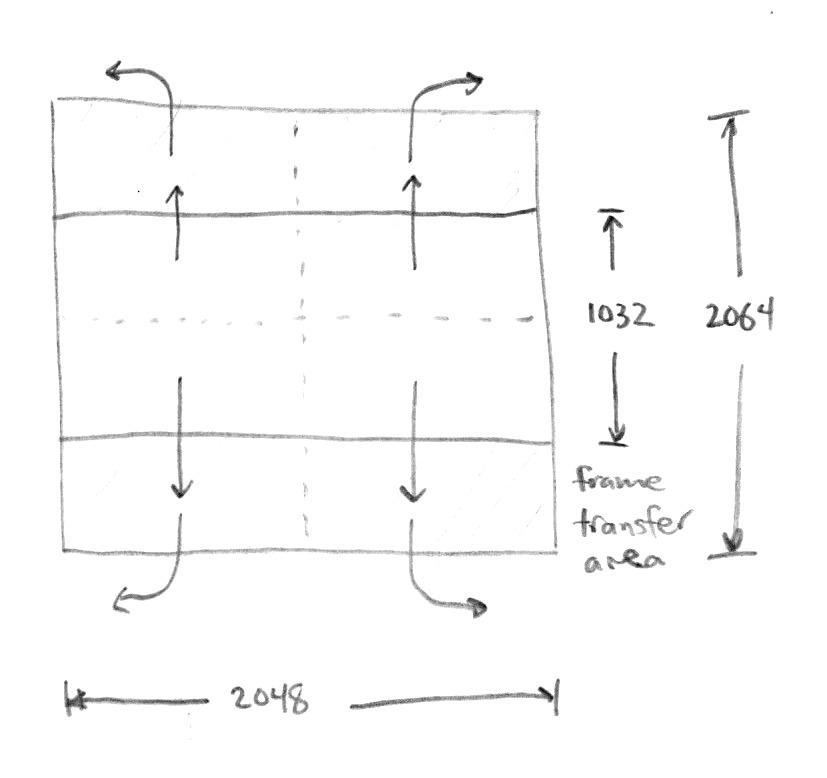
\includegraphics[width=0.4\textwidth]{gfa-metrology2.jpeg}
  \end{center}
  \caption{\label{fig:mountain}Readout of the GFA CCDs on the
    mountain, showing the masked region.  The \code{gfa} files include
    prescan and overscan columns, not shown here.}
\end{figure}

In the notebook \code{gfa-metrology.ipynb}, we copy-paste the results
cells from each of the GFA metrology reports, and also extract the
images, then go through each image and detect and measure the spot
location to sub-pixel accuracy, by fitting a 2-d Gaussian profile (and
masking saturated pixels).  We transform these measurements to
coordinates that match the spreadsheet coordinate system, and also
transform to match the mountain coordinate system.  We then fit a
linear transformation from the mountain pixel coordinate system (in
FITS-indexed pixels), to millimeters.

Finally, we copy-paste the GIF measured pinhole locations, and apply
the transformation to report those positions in GFA pixel positions.

\paragraph{Output files}

The \code{gfa-metrology-transform.fits} file contains columns:
\begin{itemize}
\item{gfa\_num} GFA\#x identifier
\item{pix\_x\_coeffs, pix\_y\_coeffs} millimeters-to-mountain-pixel x and y transformations, as (offset, x, y).
\item{mm\_x\_coeffs, mm\_y\_coeffs} mountain-pixels-to-millimeters x and y transformations, as (offset, x, y).
\item{gif\_1\_mm\_x, gif\_1\_mm\_y} GIF 1, millimeter coordinates
\item{gif\_2\_mm\_x, gif\_2\_mm\_y} GIF 2, millimeter coordinates
\item{gif\_1\_pix\_x, gif\_1\_pix\_y} GIF 1, millimeter coordinates transformed
  into mountain pixel coordinates.
\item{gif\_1\_pix\_x, gif\_1\_pix\_y} GIF 2, millimeter coordinates transformed
  into mountain pixel coordinates.
\end{itemize}


\paragraph{Notes}

Some of the spreadsheet filenames end in \code{.fit} while the actual
filenames are \code{.fits}.

GFA\#2 has a transcription error in one of the spot positions: the
spreadsheet contains $1548$, but the measured position is $\sim 1458$.

GFA\#4 \emph{was} missing file \code{IMG\_30.fits} in version
DESI-4822-v2; it exists in DESI-4822-v3.

The spots are saturated in some images.










\end{document}
